% Caption format: all caption text italic; Figure label bold italic.
\providecommand{\roomfourfigurecaption}[2]{%
  \par\smallskip
  \noindent\begin{minipage}{\textwidth}%
  \textit{\textbf{Figure #1.} #2}%
  \end{minipage}\par\smallskip
}


\section{Object Oriented Design}

\subsection{Domain model}

\par\medskip
\begin{center}
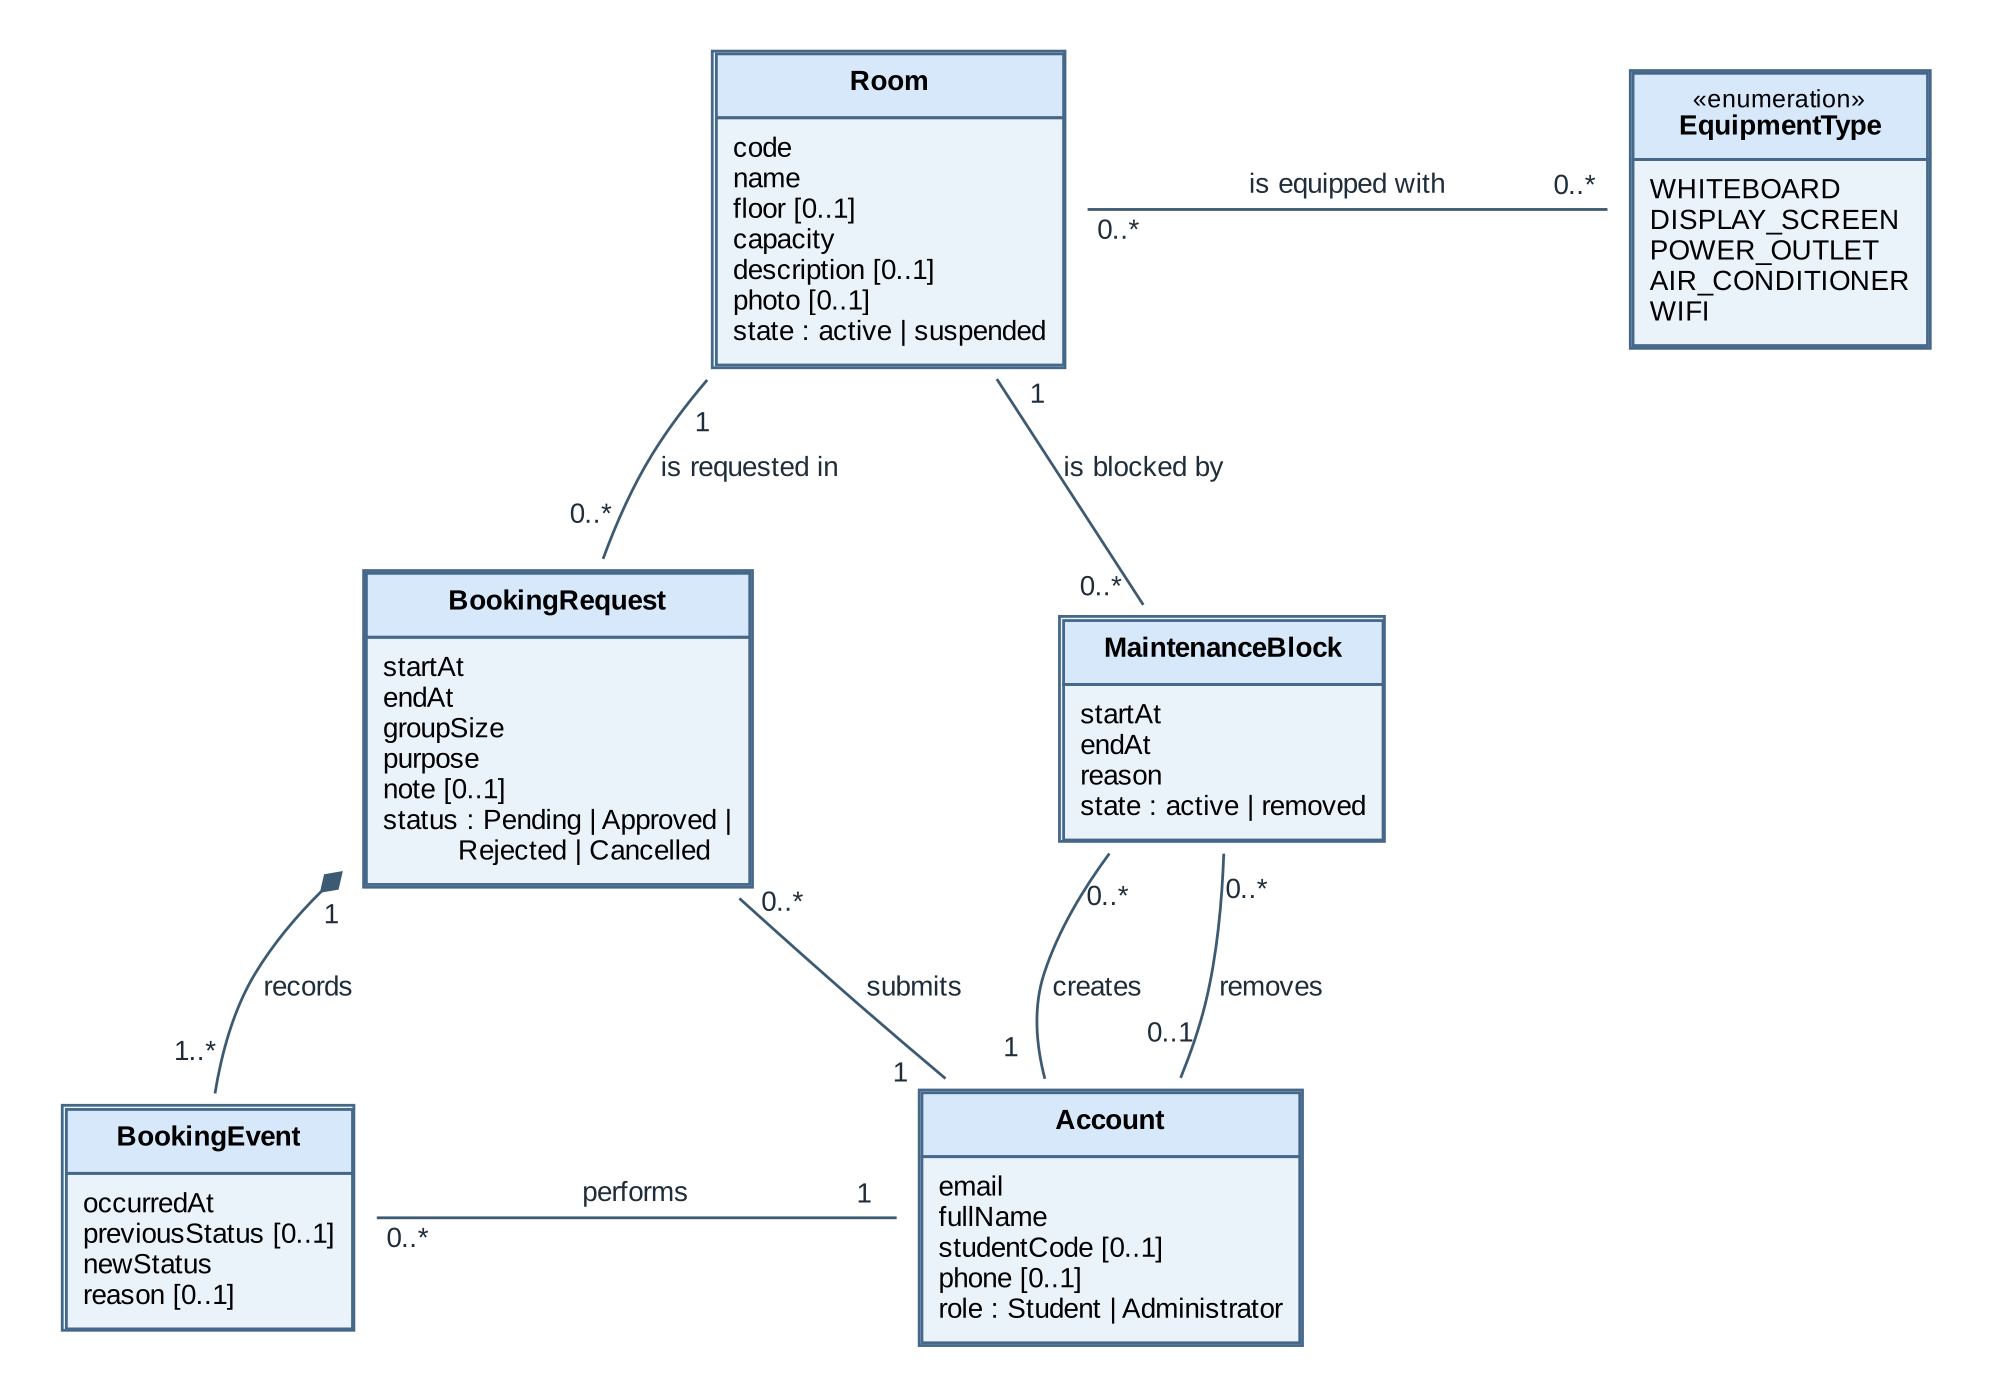
\includegraphics[width=0.94\textwidth,height=0.60\textheight,keepaspectratio]{images/05-object-oriented-design/figure_01.png}
\end{center}
\roomfourfigurecaption{U01}{Conceptual domain model. Attributes name business concepts only; identifiers, foreign keys and operations are deliberately omitted.}
\par\medskip

Role is data, not inheritance. Student and Administrator accounts carry the same identity and profile data and differ only in permissions, which Room4U checks on the server (ADR-003). Only a Student owns requests; only an Administrator creates or removes maintenance blocks and records review transitions.\par

One request, one lifecycle. A BookingRequest becomes a booking when its status is Approved; it is not copied into a second Booking entity (BR-09, BR-12). Each request has one owner and one room; a room receives many requests over time.\par

History is part of the request. BookingEvent is a composition part of its request: one event is created with the request and one for every later status change, and events are never edited or deleted (FR-19, BR-16).\par

Fixed catalogues. Equipment types and purpose codes are fixed ADR-005 catalogues, not records that users manage. A room may have no equipment.\par

Technical data is excluded. room\_occupancy (DB01) is a persistence projection, not a business concept. "Occupies an interval" follows from Approved status or an active block, and "under maintenance" is derived from active blocks rather than stored as a third room state.\par

\subsection{Design class diagrams}

\par\medskip
\begin{center}
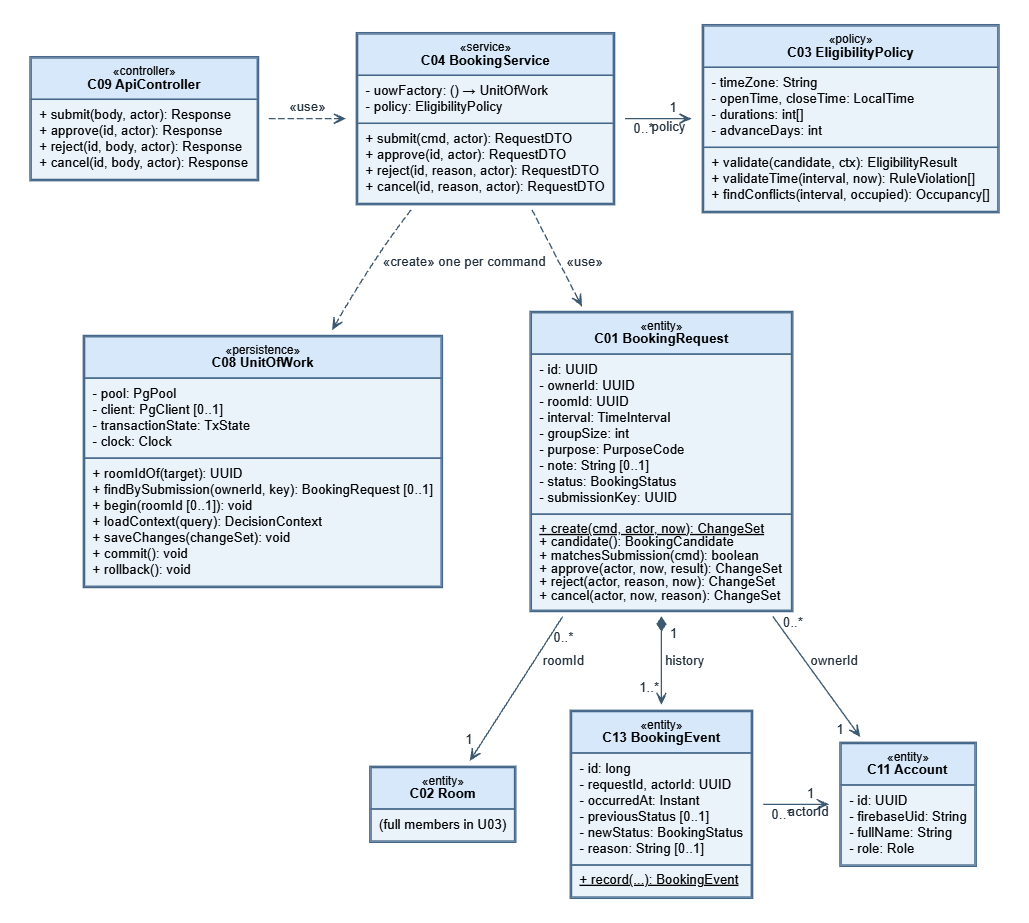
\includegraphics[width=0.94\textwidth,height=0.60\textheight,keepaspectratio]{images/05-object-oriented-design/figure_02.png}
\end{center}
\roomfourfigurecaption{U02}{Booking command package (M04, M06, M07). Services create one UnitOfWork per command; entities stage changes but never execute SQL.}
\par\medskip

C09 passes the server-injected AuthContext; it never reads a role or owner ID from request JSON. C04 holds one shared, stateless C03 and obtains a fresh C08 from its factory for each command. C01 enforces its own transitions and returns a ChangeSet that contains the status change, any occupancy row to add or delete and exactly one C13 event created through record() . Associations to C02 and C11 are ID references (roomId, ownerId), so a command does not need to load a whole object graph.\par

\par\medskip
\begin{center}
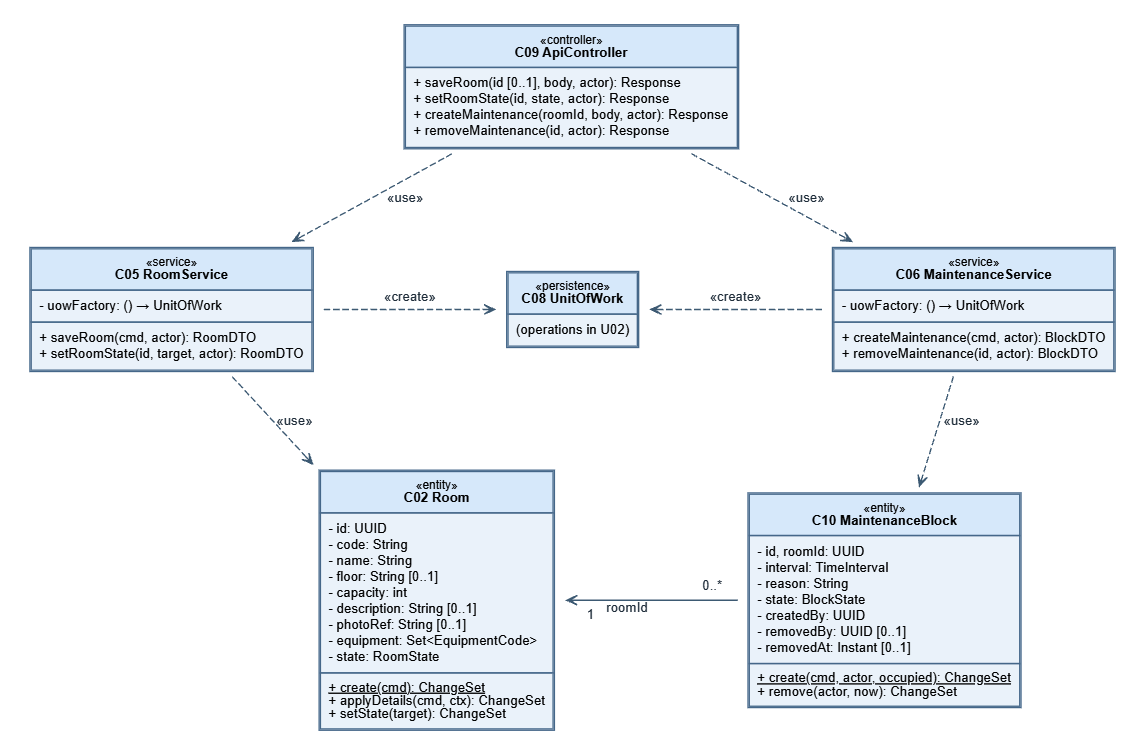
\includegraphics[width=0.94\textwidth,height=0.60\textheight,keepaspectratio]{images/05-object-oriented-design/figure_03.png}
\end{center}
\roomfourfigurecaption{U03}{Room and maintenance command package (M05). C05 and C06 use the same C08 room guard as booking commands.}
\par\medskip

C02.applyDetails receives the decision context read after the room lock: the largest group size among the room's future Approved bookings and whether the normalized code already belongs to another room. C10.create receives the room's current occupancy and refuses any overlap; C10.remove requires an active block whose start is still in the future. Neither service cancels a booking as a side effect.\par

\par\medskip
\begin{center}
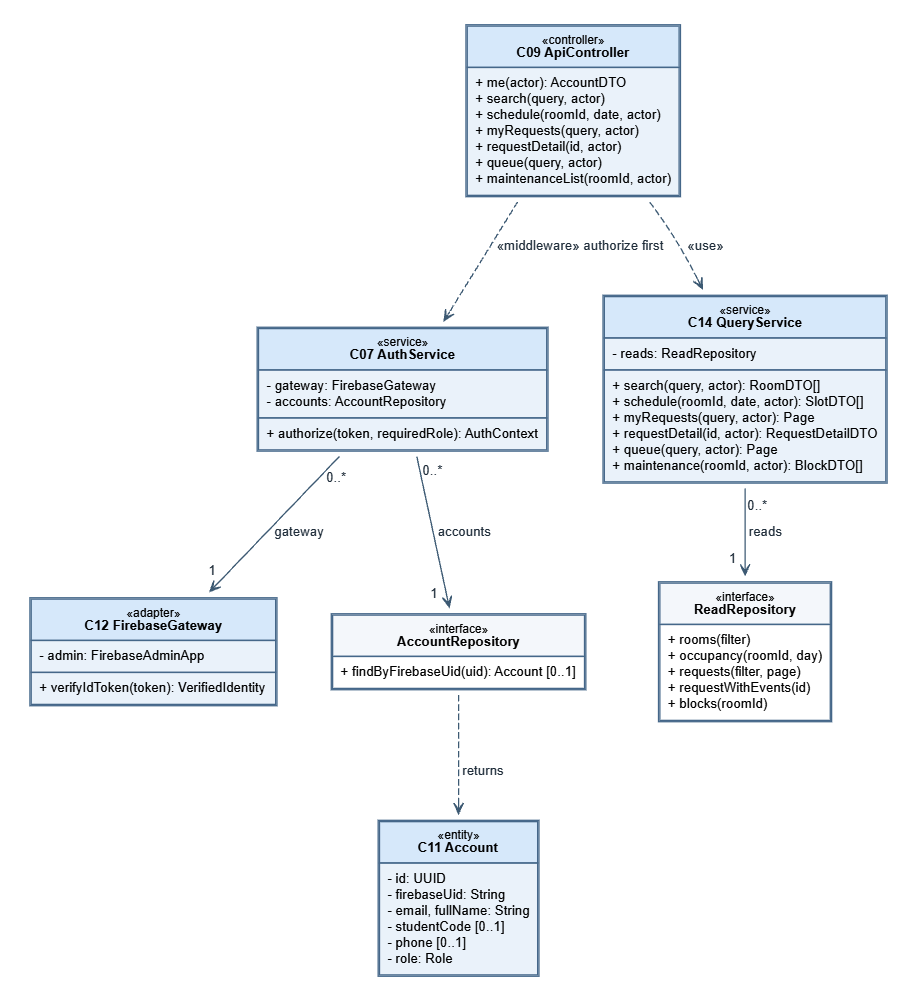
\includegraphics[width=0.94\textwidth,height=0.60\textheight,keepaspectratio]{images/05-object-oriented-design/figure_04.png}
\end{center}
\roomfourfigurecaption{U04}{Access and query package (M01, M03). Authorization runs before dispatch; read services return explicit DTO projections.}
\par\medskip

C09 invokes C07.authorize as middleware before every protected operation. C12 is the only class that imports the Firebase Admin SDK. AccountRepository and ReadRepository are interfaces implemented in the persistence component, so C07 and C14 can be verified with in-memory fakes. C14 checks owner or Administrator access for request details and returns only allow-listed fields; a shared schedule slot contains roomId, startAt, endAt and occupancy type, never an owner or a reason.\par

\subsection{Class specifications}

\subsubsection{C01 BookingRequest}

Domain entity for one student request and its allowed status transitions. No superclass.\par

\small
\setlength{\tabcolsep}{3pt}
\renewcommand{\arraystretch}{1.12}
\begin{longtable}{|p{0.14\textwidth}|p{0.17\textwidth}|p{0.16\textwidth}|p{0.24\textwidth}|p{0.21\textwidth}|}
\hline
\textbf{Attribute} & \textbf{Type} & \textbf{Visibility} & \textbf{Constraint} & \textbf{Description} \\ \hline
\endfirsthead \hline
id & UUID & private & Primary key; immutable & Stable request identity. \\ \hline
ownerId & UUID & private & Student from AuthContext; immutable & Request owner (BR-01). \\ \hline
roomId & UUID & private & Immutable (BR-12) & Requested room; also locates the room guard. \\ \hline
interval & TimeInterval & private & endAt = startAt + duration; never edited & Requested or booked half-open interval. \\ \hline
groupSize & int & private & 1 … room capacity at submission and approval (BR-05) & Number of group members. \\ \hline
purpose & PurposeCode & private & Required; ADR-005 codes & Booking purpose; no eligibility effect. \\ \hline
note & String [0..1] & private & Trimmed; ≤ 250; blank stored as null & Optional booking note. \\ \hline
status & BookingStatus & private & Changed only by the operations below & Lifecycle state. \\ \hline
submissionKey & UUID & private & Unique per owner & Replay key of one logical submission (ADR-004). \\ \hline
createdAt / updatedAt & Instant & private & Server time & Creation order and latest transition. \\ \hline
\end{longtable}
\normalsize

\small
\setlength{\tabcolsep}{3pt}
\renewcommand{\arraystretch}{1.12}
\begin{longtable}{|p{0.18\textwidth}|p{0.24\textwidth}|p{0.22\textwidth}|p{0.28\textwidth}|}
\hline
\textbf{Operation} & \textbf{Parameters → return} & \textbf{Visibility} & \textbf{Responsibility} \\ \hline
\endfirsthead \hline
create (static) & cmd: SubmitCommand, actor, now: Instant → ChangeSet & public & Builds a Pending request and its creation event (previousStatus null). Called only after an eligible C03 result; adds no occupancy (BR-07). \\ \hline
candidate & () → BookingCandidate & public & Returns room, interval and group size for re-validation at approval. \\ \hline
matchesSubmission & cmd: SubmitCommand → boolean & public & Compares the canonical submitted values (room, start, duration, group size, purpose, normalized note) for a replay. \\ \hline
approve & actor, now: Instant, result: EligibilityResult → ChangeSet & public & Requires status Pending and result.eligible. Stages Approved, one occupancy row for (roomId, interval) and one event; otherwise returns a refusal and stages nothing. \\ \hline
reject & actor, reason: String, now: Instant → ChangeSet & public & Administrator; status Pending, also after its start; reason trimmed 1–250 (BR-13). Stages Rejected and an event with the reason. \\ \hline
cancel & actor, now: Instant, reason: String [0..1] → ChangeSet & public & Owner: Pending or Approved and now < startAt. Administrator: Approved, now < startAt and reason 1–250 (BR-10). Stages Cancelled, deletes its own occupancy row when Approved and adds one event. Another student → NOT\_OWNER (403). \\ \hline
\end{longtable}
\normalsize

\subsubsection{C02 Room}

Domain entity for room details, equipment set and active/suspended state. No superclass.\par

\small
\setlength{\tabcolsep}{3pt}
\renewcommand{\arraystretch}{1.12}
\begin{longtable}{|p{0.14\textwidth}|p{0.17\textwidth}|p{0.16\textwidth}|p{0.24\textwidth}|p{0.21\textwidth}|}
\hline
\textbf{Attribute} & \textbf{Type} & \textbf{Visibility} & \textbf{Constraint} & \textbf{Description} \\ \hline
\endfirsthead \hline
id & UUID & private & Stable; immutable & Internal identity, distinct from the editable code. \\ \hline
code & String & private & Trimmed; unique ignoring case (BR-14) & User-facing room code. \\ \hline
name & String & private & Trimmed length 1–80 & Display name. \\ \hline
floor & String [0..1] & private & No fixed enumeration & Floor shown in details and filters. \\ \hline
capacity & int & private & 1–50; ≥ every future Approved group & Current capacity. \\ \hline
description & String [0..1] & private & ≤ 250 characters & Optional description. \\ \hline
photoRef & String [0..1] & private & Preloaded image; null → placeholder & Room photo reference. \\ \hline
equipment & Set<\allowbreak EquipmentCode> & private & ADR-005 codes; may be empty & Selected equipment (room\_equipment rows). \\ \hline
state & RoomState & private & active / suspended & Eligibility gate; not a booking status. \\ \hline
\end{longtable}
\normalsize

\small
\setlength{\tabcolsep}{3pt}
\renewcommand{\arraystretch}{1.12}
\begin{longtable}{|p{0.18\textwidth}|p{0.24\textwidth}|p{0.22\textwidth}|p{0.28\textwidth}|}
\hline
\textbf{Operation} & \textbf{Parameters → return} & \textbf{Visibility} & \textbf{Responsibility} \\ \hline
\endfirsthead \hline
create (static) & cmd: RoomCommand → ChangeSet & public & Validates fields and codes, assigns a new stable ID and stages an active room with its equipment rows (FR-20). The normalized unique index rejects a duplicate code at save. \\ \hline
applyDetails & cmd: RoomCommand, ctx: DecisionContext → ChangeSet & public & Validates fields; refuses a code used by another room (ctx.codeInUse) or capacity < ctx.maxFutureGroup (BR-14). Stages the detail update and, when supplied, replaces the whole equipment set. The ID never changes (FR-21). \\ \hline
setState & target: RoomState → ChangeSet & public & Allows only active → suspended and suspended → active. Never changes bookings, blocks or occupancy (BR-11). \\ \hline
\end{longtable}
\normalsize

\subsubsection{C03 EligibilityPolicy}

Stateless implementation of UC-14 used by submission and approval. It reads only the supplied context and never writes. No superclass.\par

\small
\setlength{\tabcolsep}{3pt}
\renewcommand{\arraystretch}{1.12}
\begin{longtable}{|p{0.14\textwidth}|p{0.17\textwidth}|p{0.16\textwidth}|p{0.24\textwidth}|p{0.21\textwidth}|}
\hline
\textbf{Attribute} & \textbf{Type} & \textbf{Visibility} & \textbf{Constraint} & \textbf{Description} \\ \hline
\endfirsthead \hline
timeZone & String & private & Asia/Ho\_Chi\_Minh & Local date and opening-hour interpretation. \\ \hline
openTime / closeTime & LocalTime & private & 08:00 / 20:00 & Booking window on one local date (BR-02). \\ \hline
durations & int[] & private & \{30, 60, 90, 120\} & Allowed durations in minutes (BR-03). \\ \hline
startStep\allowbreak Minutes & int & private & 30 & Start on :00 or :30 with zero seconds. \\ \hline
advanceDays & int & private & 7; rolling instant boundary & Maximum advance period (BR-04). \\ \hline
\end{longtable}
\normalsize

\small
\setlength{\tabcolsep}{3pt}
\renewcommand{\arraystretch}{1.12}
\begin{longtable}{|p{0.18\textwidth}|p{0.24\textwidth}|p{0.22\textwidth}|p{0.28\textwidth}|}
\hline
\textbf{Operation} & \textbf{Parameters → return} & \textbf{Visibility} & \textbf{Responsibility} \\ \hline
\endfirsthead \hline
validate & candidate: BookingCandidate, ctx: DecisionContext → EligibilityResult & public & Collects all violations: room active (BR-11), validateTime, 1 ≤ groupSize ≤ ctx room capacity (BR-05) and no conflict from findConflicts (BR-06–08). \\ \hline
validateTime & interval: TimeInterval, now: Instant → RuleViolation[] & public & Start step, allowed duration, same local date inside 08:00–20:00 (end at 20:00 allowed) and now < start ≤ now + 7 days. \\ \hline
findConflicts & interval: TimeInterval, occupied: Occupancy[] → Occupancy[] & public & Returns Approved or maintenance occupancy that overlaps the interval. Pending requests are never in occupied (BR-07). \\ \hline
\end{longtable}
\normalsize

\subsubsection{C04 BookingService}

Coordinates submission, approval, rejection and cancellation (UC-04, UC-06, UC-08–UC-10). No superclass.\par

\small
\setlength{\tabcolsep}{3pt}
\renewcommand{\arraystretch}{1.12}
\begin{longtable}{|p{0.14\textwidth}|p{0.17\textwidth}|p{0.16\textwidth}|p{0.24\textwidth}|p{0.21\textwidth}|}
\hline
\textbf{Attribute} & \textbf{Type} & \textbf{Visibility} & \textbf{Constraint} & \textbf{Description} \\ \hline
\endfirsthead \hline
uowFactory & () → UnitOfWork & private & New unit per command & Never shares a transaction client between requests. \\ \hline
policy & EligibilityPolicy & private & Injected; shared; stateless & UC-14 rules. \\ \hline
\end{longtable}
\normalsize

\small
\setlength{\tabcolsep}{3pt}
\renewcommand{\arraystretch}{1.12}
\begin{longtable}{|p{0.18\textwidth}|p{0.24\textwidth}|p{0.22\textwidth}|p{0.28\textwidth}|}
\hline
\textbf{Operation} & \textbf{Parameters → return} & \textbf{Visibility} & \textbf{Responsibility} \\ \hline
\endfirsthead \hline
submit & cmd: SubmitCommand, actor → RequestDTO & public & Student. Replay check by owner/key (200 same values, 409 different). If no request is found, lock the room and repeat the owner/key lookup before running UC-14; a hit rolls back and is answered as a replay. Otherwise load ctx, validate, C01.create, save and commit → 201 Pending. A unique-key conflict at save rolls back, rereads the stored request and is answered as a replay. \\ \hline
approve & id: UUID, actor → RequestDTO & public & Administrator. roomIdOf, lock, reload request and occupancy, validate, C01.approve, save, commit. Request no longer Pending → rollback, 409 with its current status. Pending but not eligible, or an exclusion violation (23P01) → rollback, 409 with the causes; the request stays Pending. \\ \hline
reject & id: UUID, reason: String, actor → RequestDTO & public & Administrator. Same guard; C01.reject; no occupancy change. \\ \hline
cancel & id: UUID, reason: String [0..1], actor → RequestDTO & public & Owner (UC-06) or Administrator (UC-10). Same guard; C01.cancel; releases only this request's occupancy. \\ \hline
\end{longtable}
\normalsize

\subsubsection{C05 RoomService}

Creates and edits rooms and changes room state (UC-11, UC-12). No superclass.\par

\small
\setlength{\tabcolsep}{3pt}
\renewcommand{\arraystretch}{1.12}
\begin{longtable}{|p{0.14\textwidth}|p{0.17\textwidth}|p{0.16\textwidth}|p{0.24\textwidth}|p{0.21\textwidth}|}
\hline
\textbf{Attribute} & \textbf{Type} & \textbf{Visibility} & \textbf{Constraint} & \textbf{Description} \\ \hline
\endfirsthead \hline
uowFactory & () → UnitOfWork & private & New unit per command & Transaction and room guard. \\ \hline
\end{longtable}
\normalsize

\small
\setlength{\tabcolsep}{3pt}
\renewcommand{\arraystretch}{1.12}
\begin{longtable}{|p{0.18\textwidth}|p{0.24\textwidth}|p{0.22\textwidth}|p{0.28\textwidth}|}
\hline
\textbf{Operation} & \textbf{Parameters → return} & \textbf{Visibility} & \textbf{Responsibility} \\ \hline
\endfirsthead \hline
saveRoom & cmd: RoomCommand, actor → RoomDTO & public & Administrator. New room: begin(null), C02.create, save, commit; duplicate normalized code (23505) → 409. Existing room: begin(roomId), loadContext, C02.applyDetails, save, commit (SQ04). \\ \hline
setRoomState & id: UUID, target: RoomState, actor → RoomDTO & public & Administrator. begin(id), reread state, C02.setState, save, commit. Existing bookings and blocks stay unchanged. \\ \hline
\end{longtable}
\normalsize

\subsubsection{C06 MaintenanceService}

Creates maintenance blocks and removes future blocks (UC-13). No superclass.\par

\small
\setlength{\tabcolsep}{3pt}
\renewcommand{\arraystretch}{1.12}
\begin{longtable}{|p{0.14\textwidth}|p{0.17\textwidth}|p{0.16\textwidth}|p{0.24\textwidth}|p{0.21\textwidth}|}
\hline
\textbf{Attribute} & \textbf{Type} & \textbf{Visibility} & \textbf{Constraint} & \textbf{Description} \\ \hline
\endfirsthead \hline
uowFactory & () → UnitOfWork & private & New unit per command & Same room guard as approval. \\ \hline
\end{longtable}
\normalsize

\small
\setlength{\tabcolsep}{3pt}
\renewcommand{\arraystretch}{1.12}
\begin{longtable}{|p{0.18\textwidth}|p{0.24\textwidth}|p{0.22\textwidth}|p{0.28\textwidth}|}
\hline
\textbf{Operation} & \textbf{Parameters → return} & \textbf{Visibility} & \textbf{Responsibility} \\ \hline
\endfirsthead \hline
createMaintenance & cmd: BlockCommand, actor → BlockDTO & public & Administrator. begin(roomId), load occupancy, C10.create, save, commit. On overlap, roll back and return 409 with code SCHEDULE\_CONFLICT, requestId and conflicts. Following SQ05, list overlapping Approved bookings first (kind = approved\_booking, bookingRequestId, startAt, endAt); only if none overlap, return the active maintenance conflict (kind = maintenance\_block, maintenanceBlockId, startAt, endAt). S08 links bookings to UC-10; no booking is cancelled automatically (BR-15). \\ \hline
removeMaintenance & id: UUID, actor → BlockDTO & public & Administrator. roomIdOf(block), begin, reload block, C10.remove(actor, ctx.now), save, commit. The block record is kept (FR-26). \\ \hline
\end{longtable}
\normalsize

\subsubsection{C07 AuthService}

Verifies identity and resolves the application role before any protected behavior. No superclass.\par

\small
\setlength{\tabcolsep}{3pt}
\renewcommand{\arraystretch}{1.12}
\begin{longtable}{|p{0.14\textwidth}|p{0.17\textwidth}|p{0.16\textwidth}|p{0.24\textwidth}|p{0.21\textwidth}|}
\hline
\textbf{Attribute} & \textbf{Type} & \textbf{Visibility} & \textbf{Constraint} & \textbf{Description} \\ \hline
\endfirsthead \hline
gateway & FirebaseGateway & private & Adapter over Firebase Admin SDK & Verifies ID tokens. \\ \hline
accounts & AccountRepository & private & Read-only & Maps firebaseUid to the internal account and role. \\ \hline
\end{longtable}
\normalsize

\small
\setlength{\tabcolsep}{3pt}
\renewcommand{\arraystretch}{1.12}
\begin{longtable}{|p{0.18\textwidth}|p{0.24\textwidth}|p{0.22\textwidth}|p{0.28\textwidth}|}
\hline
\textbf{Operation} & \textbf{Parameters → return} & \textbf{Visibility} & \textbf{Responsibility} \\ \hline
\endfirsthead \hline
authorize & token: String, requiredRole: Role [0..1] → AuthContext & public & Invalid or expired token, or no matching account → 401; role differs from requiredRole → 403. Returns only \{userId, role\} from the users row. Runs before dispatch, so no Firebase call happens while a room lock is held. \\ \hline
\end{longtable}
\normalsize

\subsubsection{C08 UnitOfWork}

One-command transaction and repository facade (M07). Each instance owns at most one pooled client. No superclass.\par

\small
\setlength{\tabcolsep}{3pt}
\renewcommand{\arraystretch}{1.12}
\begin{longtable}{|p{0.14\textwidth}|p{0.17\textwidth}|p{0.16\textwidth}|p{0.24\textwidth}|p{0.21\textwidth}|}
\hline
\textbf{Attribute} & \textbf{Type} & \textbf{Visibility} & \textbf{Constraint} & \textbf{Description} \\ \hline
\endfirsthead \hline
pool & PgPool & private & Configured once per process & Connection source; not the transaction itself. \\ \hline
client & PgClient [0..1] & private & One checked-out connection until commit/rollback & Every statement of the command uses this client. \\ \hline
transaction\allowbreak State & TxState & private & idle / active / committed / rolledBack & Blocks writes outside an active unit. \\ \hline
clock & Clock & private & Server clock in production; fixed clock in tests & Decision instant sampled after the lock. \\ \hline
\end{longtable}
\normalsize

\small
\setlength{\tabcolsep}{3pt}
\renewcommand{\arraystretch}{1.12}
\begin{longtable}{|p{0.18\textwidth}|p{0.24\textwidth}|p{0.22\textwidth}|p{0.28\textwidth}|}
\hline
\textbf{Operation} & \textbf{Parameters → return} & \textbf{Visibility} & \textbf{Responsibility} \\ \hline
\endfirsthead \hline
roomIdOf & target: TargetRef → UUID & public & Non-locking read of the immutable room\_id of a request or block before BEGIN; unknown target → 404. \\ \hline
findBySubmission & ownerId: UUID, key: UUID → BookingRequest [0..1] & public & Replay lookup by owner and key. Called before the submission transaction, again after the room guard is held, and after a rollback caused by a unique-key conflict. \\ \hline
begin & roomId: UUID [0..1] → void & public & BEGIN at READ COMMITTED and SELECT the rooms row FOR UPDATE. Null only for creating a new room. \\ \hline
loadContext & query: ContextQuery → DecisionContext & public & Reads current room, target, occupancy, maxFutureGroup and codeInUse as the query requests; samples now (clock\_timestamp) after the lock. \\ \hline
saveChanges & changeSet: ChangeSet → void & public & Writes source rows, occupancy projection and events with the same client. Maps 23P01 to a schedule conflict and 23505 by constraint name. \\ \hline
commit & () → void & public & COMMIT and release the client; services report success only afterwards. \\ \hline
rollback & () → void & public & ROLLBACK and release the client after any refusal or error; safe to call twice. \\ \hline
\end{longtable}
\normalsize

\subsubsection{Supporting classes C09–C14}

\small
\setlength{\tabcolsep}{2pt}
\renewcommand{\arraystretch}{1.12}
\begin{longtable}{|>{\raggedright\arraybackslash}p{0.18\textwidth}|>{\raggedright\arraybackslash}p{0.24\textwidth}|>{\raggedright\arraybackslash}p{0.22\textwidth}|>{\raggedright\arraybackslash}p{0.28\textwidth}|}
\hline
\textbf{ID} & \textbf{Class} & \textbf{Responsibility} & \textbf{Key operations} \\ \hline
\endfirsthead \hline
C09 & ApiController\allowbreak{} «controller» & Routes /api/v1, parses DTOs, runs C07 as middleware, translates domain outcomes to 401/\allowbreak 403/\allowbreak 404/\allowbreak 409/\allowbreak 422/\allowbreak 503. & As listed in U02–U04. \\ \hline
C10 & MaintenanceBlock «entity» & Block interval, reason, active/removed state, creator and remover. Removed blocks are retained. & create (static): end > start, reason trimmed 1–250, no overlap with occupied → block + occupancy (BR-13, BR-15). remove(actor, now): active and now < startAt → removed, delete own occupancy, record actor and time (FR-26). \\ \hline
C11 & Account «entity» & Pre-created account with profile fields and role; read-only in this scope. & Attributes only. \\ \hline
C12 & FirebaseGateway «adapter» & Only class that depends on the Firebase Admin SDK. & verifyIdToken(token) → VerifiedIdentity. \\ \hline
C13 & BookingEvent «entity» & Append-only transition record; never updated or deleted. & record (static): event for a creation or transition. \\ \hline
C14 & QueryService «service» & Read use cases UC-03, UC-05, UC-07 and the S08 block list through ReadRepository; owner/Administrator checks; paging. & search, schedule, myRequests, requestDetail, queue, maintenance. \\ \hline
\end{longtable}
\normalsize

\subsection{Sequence diagrams}

SQ01–SQ05 show five Must flows; arrows mark calls/returns and alt fragments show PA2 alternatives/errors. Section 4.8 defines C09 routes, C07 authorizes, and Section 4.6 governs commit/rollback.\par

\clearpage
\subsubsection{SQ01 UC-04 Submit booking request}

\begin{center}
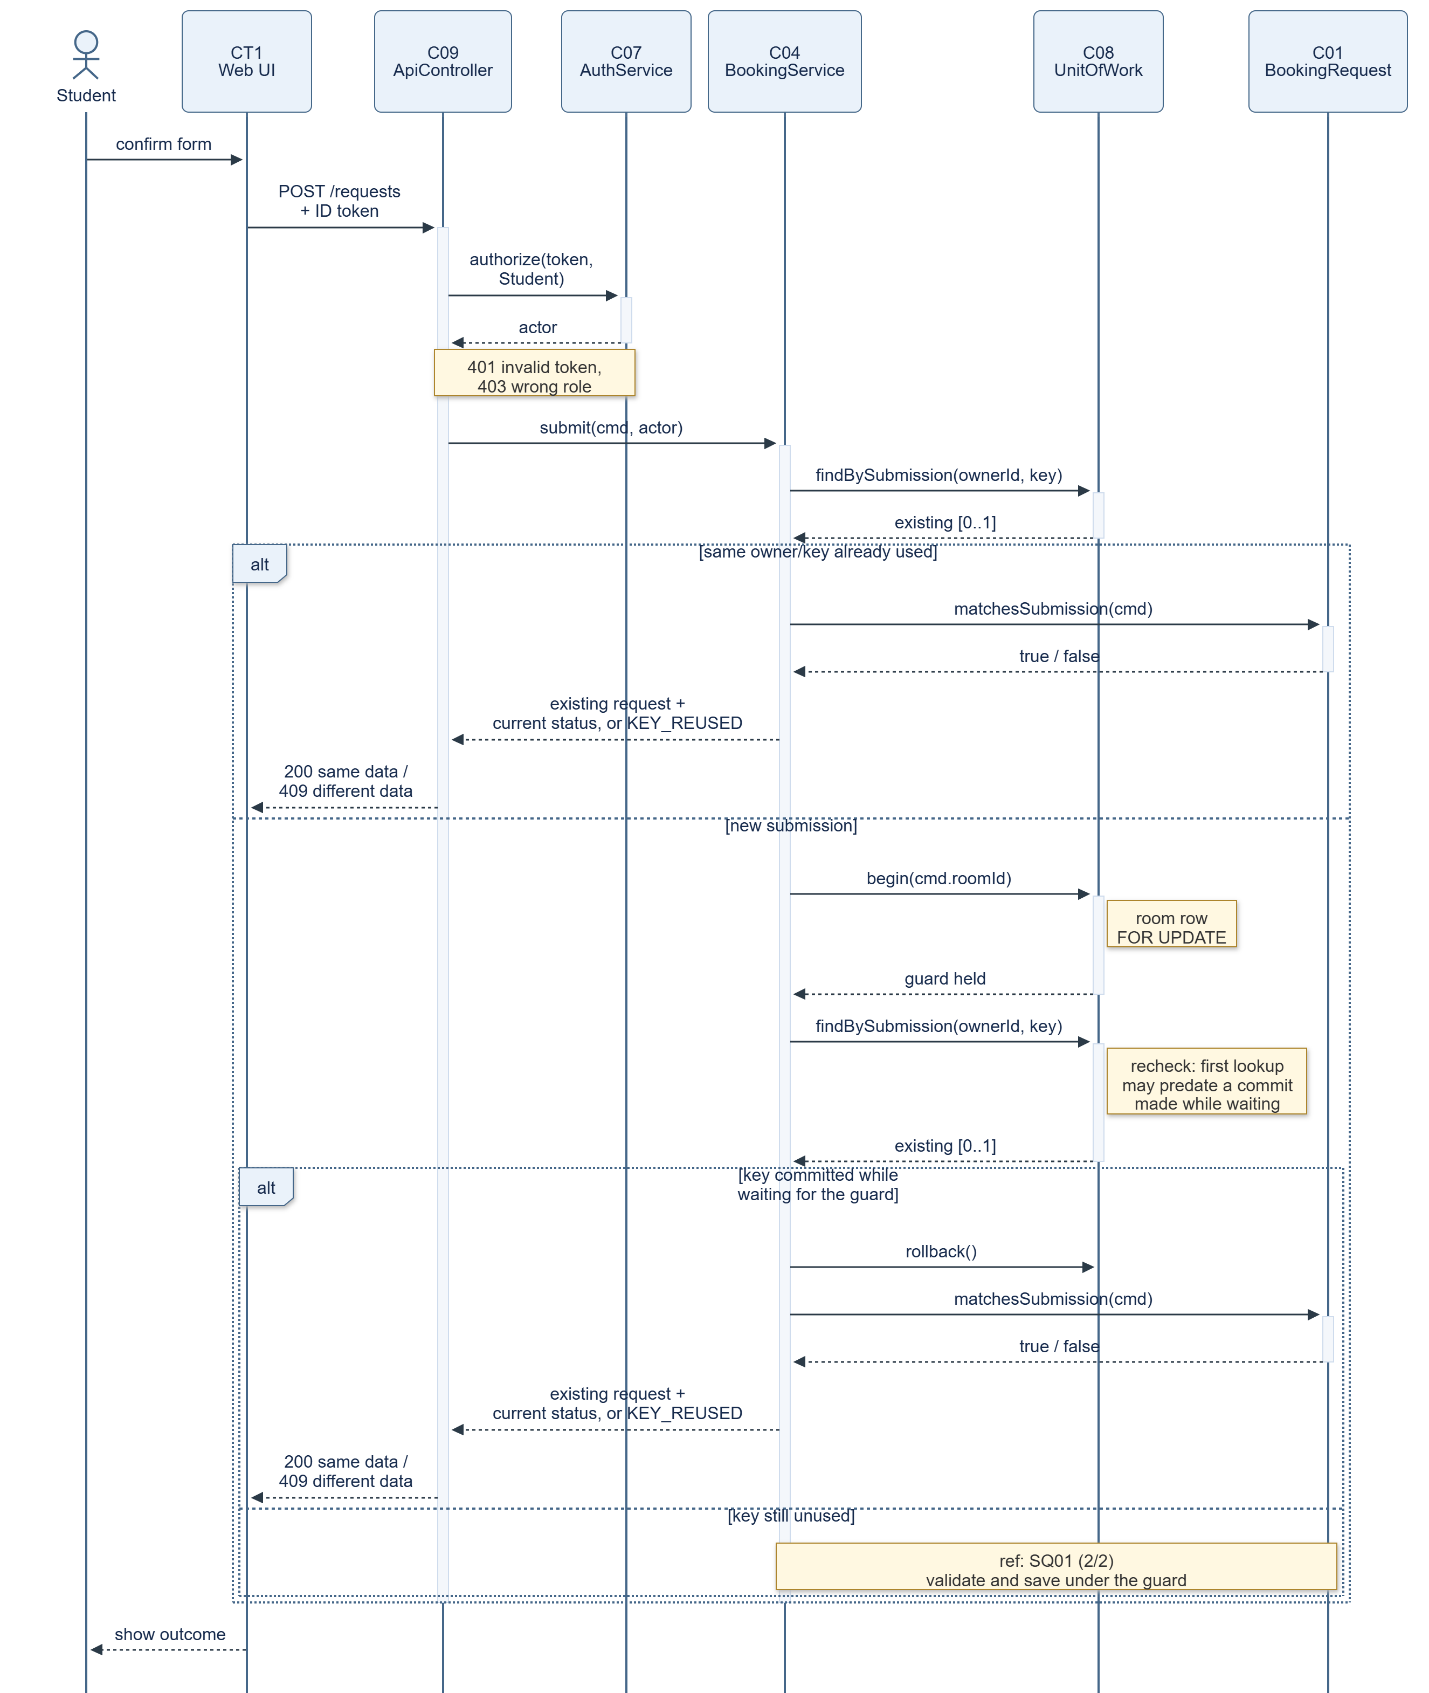
\includegraphics[width=0.98\textwidth,height=0.84\textheight,keepaspectratio]{images/05-object-oriented-design/figure_05.png}
\end{center}
\roomfourfigurecaption{SQ01a}{UC-04 submission, part 1 of 2: authorization, initial replay lookup and room-guard recheck.}

\clearpage
\begin{center}
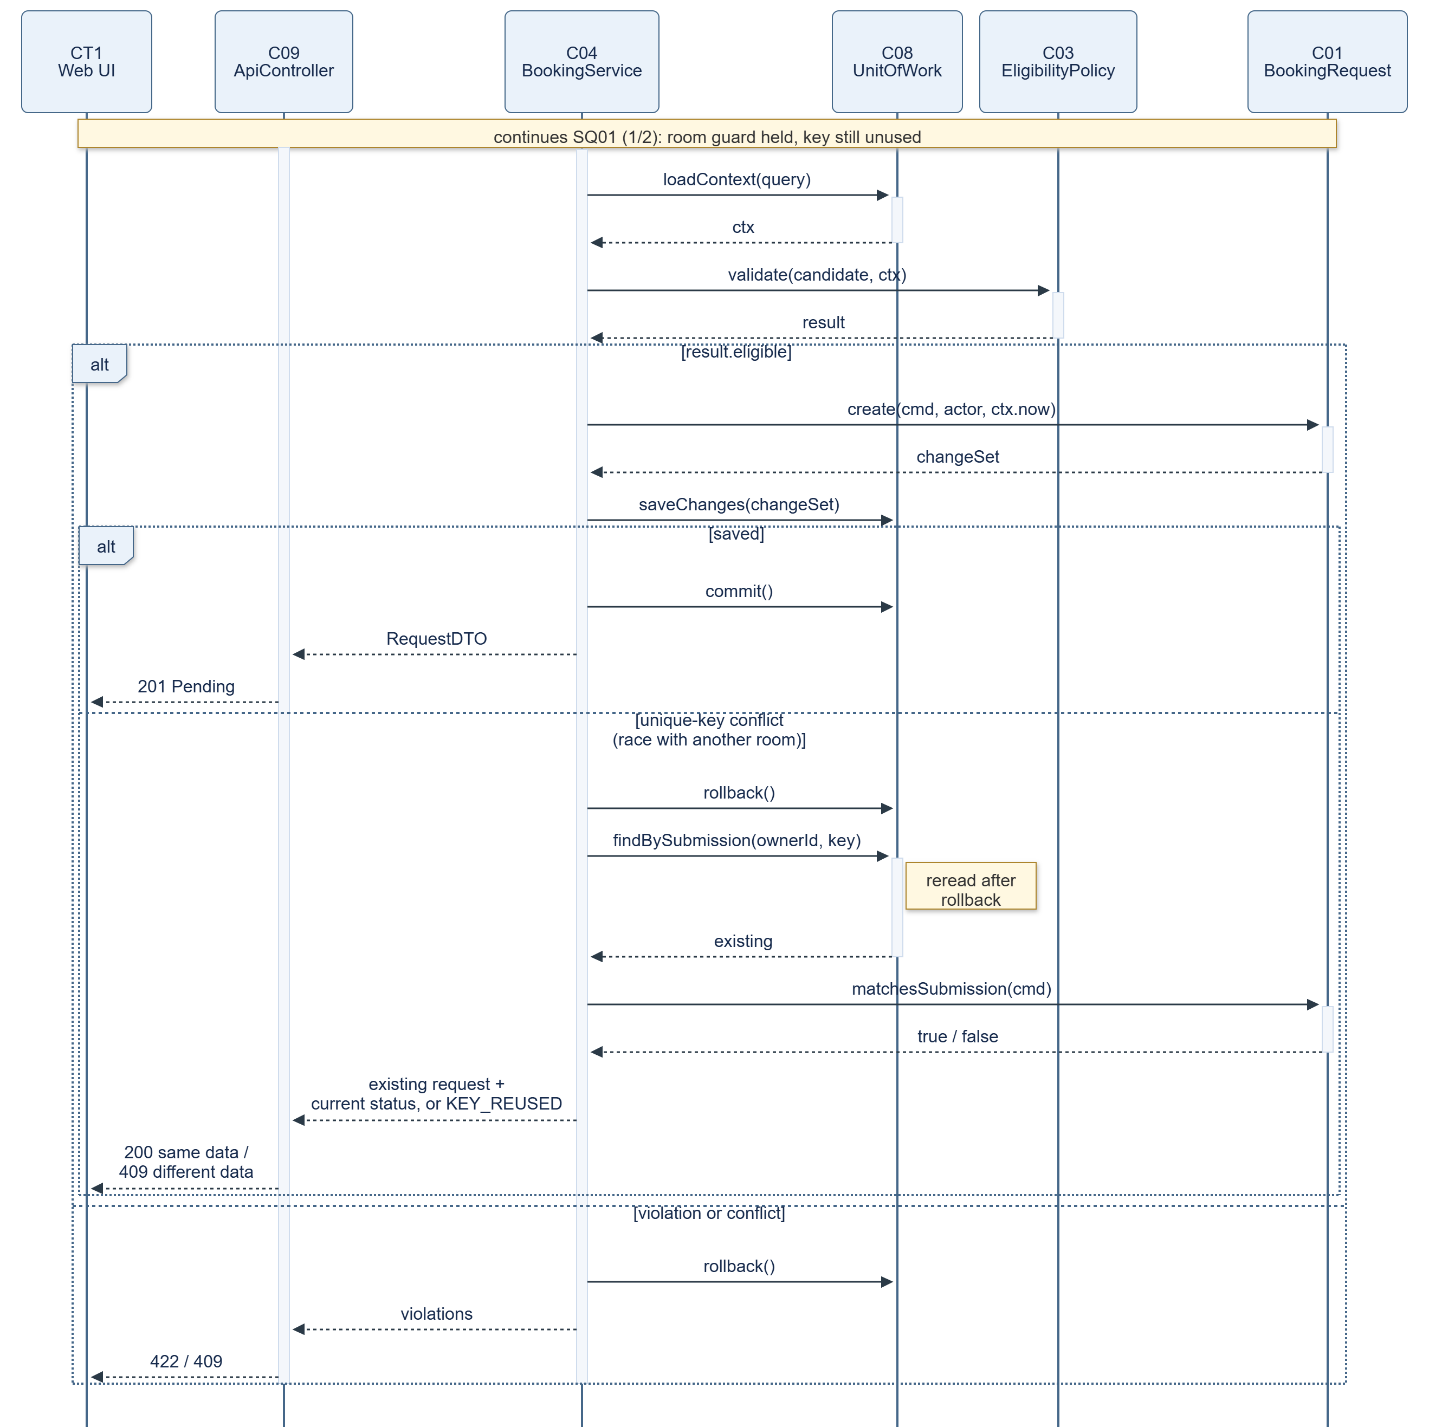
\includegraphics[width=0.98\textwidth,height=0.84\textheight,keepaspectratio]{images/05-object-oriented-design/figure_06.png}
\end{center}
\roomfourfigurecaption{SQ01b}{UC-04 submission, part 2 of 2: validation, commit and unique-key conflict handling.}
\clearpage

The replay branch runs first: the same owner and submissionKey return the existing request (200) when the canonical values match and 409 when they differ. If the first lookup finds no request, the service takes the room guard and looks up ownerId + submissionKey again before running UC-14, because a submission with the same key may have committed while this one was waiting for the guard; a hit rolls back and is answered as a replay. Only when the key is still unused does query load the locked room and its occupancy. The successful ChangeSet contains the Pending request and its creation event, with no occupancy row; overlapping Pending requests are not occupancy and never block a submission (BR-07). Field violations return 422; a suspended room or an occupied interval returns 409. A same-key submission for another room is not serialized by this guard, so the unique constraint on ownerId + submissionKey can still fail at saveChanges; the service then rolls back, rereads the stored request and handles it as a replay (200 or 409).\par

\subsubsection{SQ02 UC-08 approval}

\par\medskip
\begin{center}
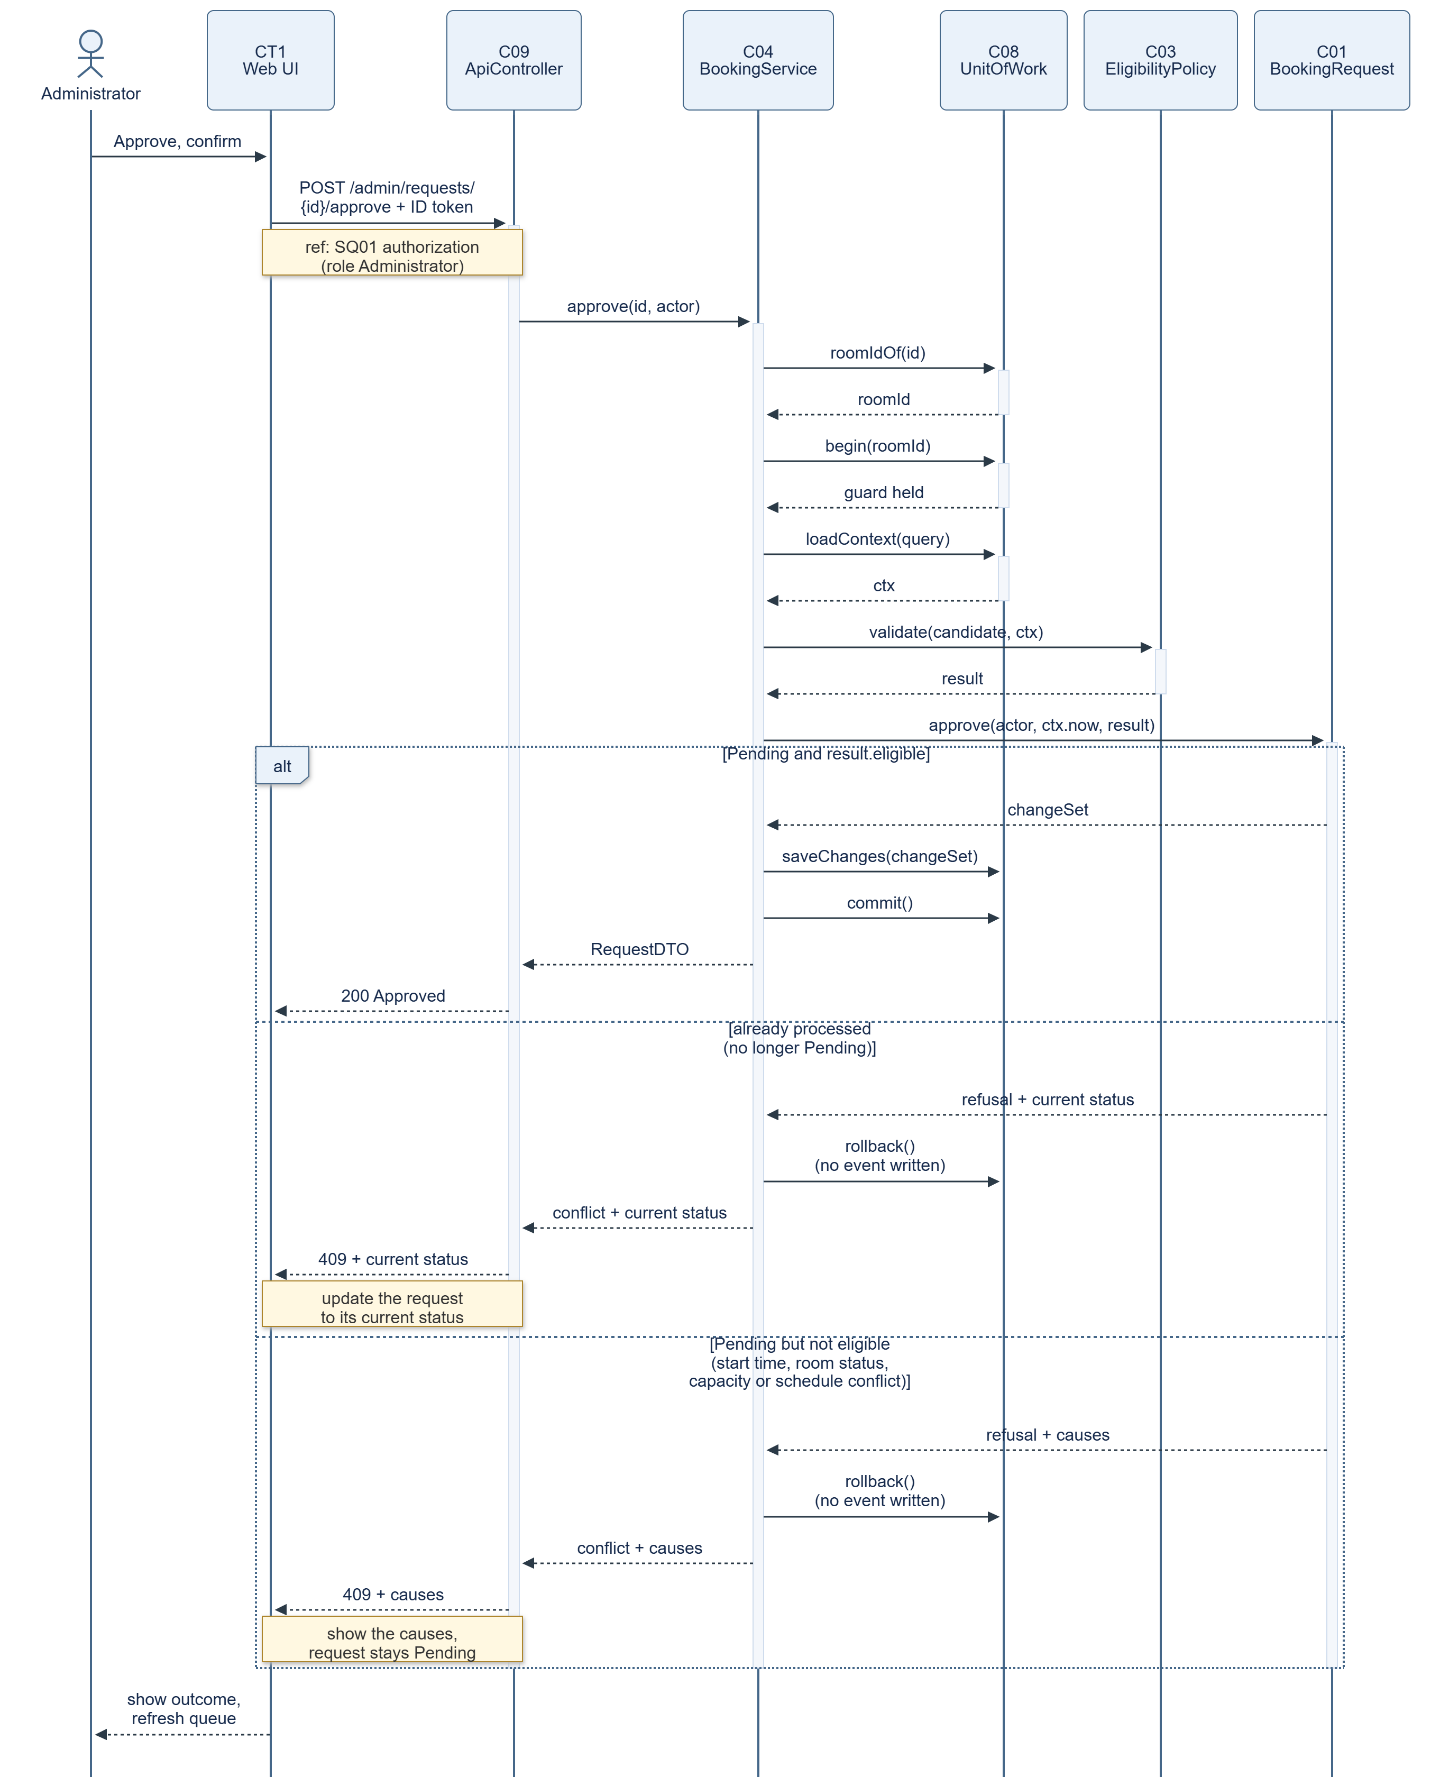
\includegraphics[width=0.94\textwidth,height=0.60\textheight,keepaspectratio]{images/05-object-oriented-design/figure_07.png}
\end{center}
\roomfourfigurecaption{SQ02}{UC-08 approval with eligibility re-evaluated after the room guard.}
\par\medskip

The service resolves the immutable room ID, takes the room guard and only then reads the request, room and occupancy. C03 rechecks time against the decision instant (BR-04 at approval), suspension, capacity and overlap; C01.approve additionally requires status Pending. The ChangeSet stages Approved, exactly one matching occupancy row and one event. A refusal has two outcomes, and neither writes an event. If the request has already been processed (approved, rejected or cancelled in the meantime), the service rolls back and returns 409 with its current status so that the UI shows that status. If the request is still Pending but not eligible, for example because a concurrent approval or maintenance command committed first and its occupancy is visible after the lock, the service rolls back and returns 409 with the causes, and the request stays Pending. The exclusion constraint (23P01) is the last safeguard and is reported as a schedule conflict in the same way. UC-09 rejection uses the same frame with C01.reject and no C03 call.\par

\subsubsection{SQ03 UC-06 Cancel own request}

\par\medskip
\begin{center}
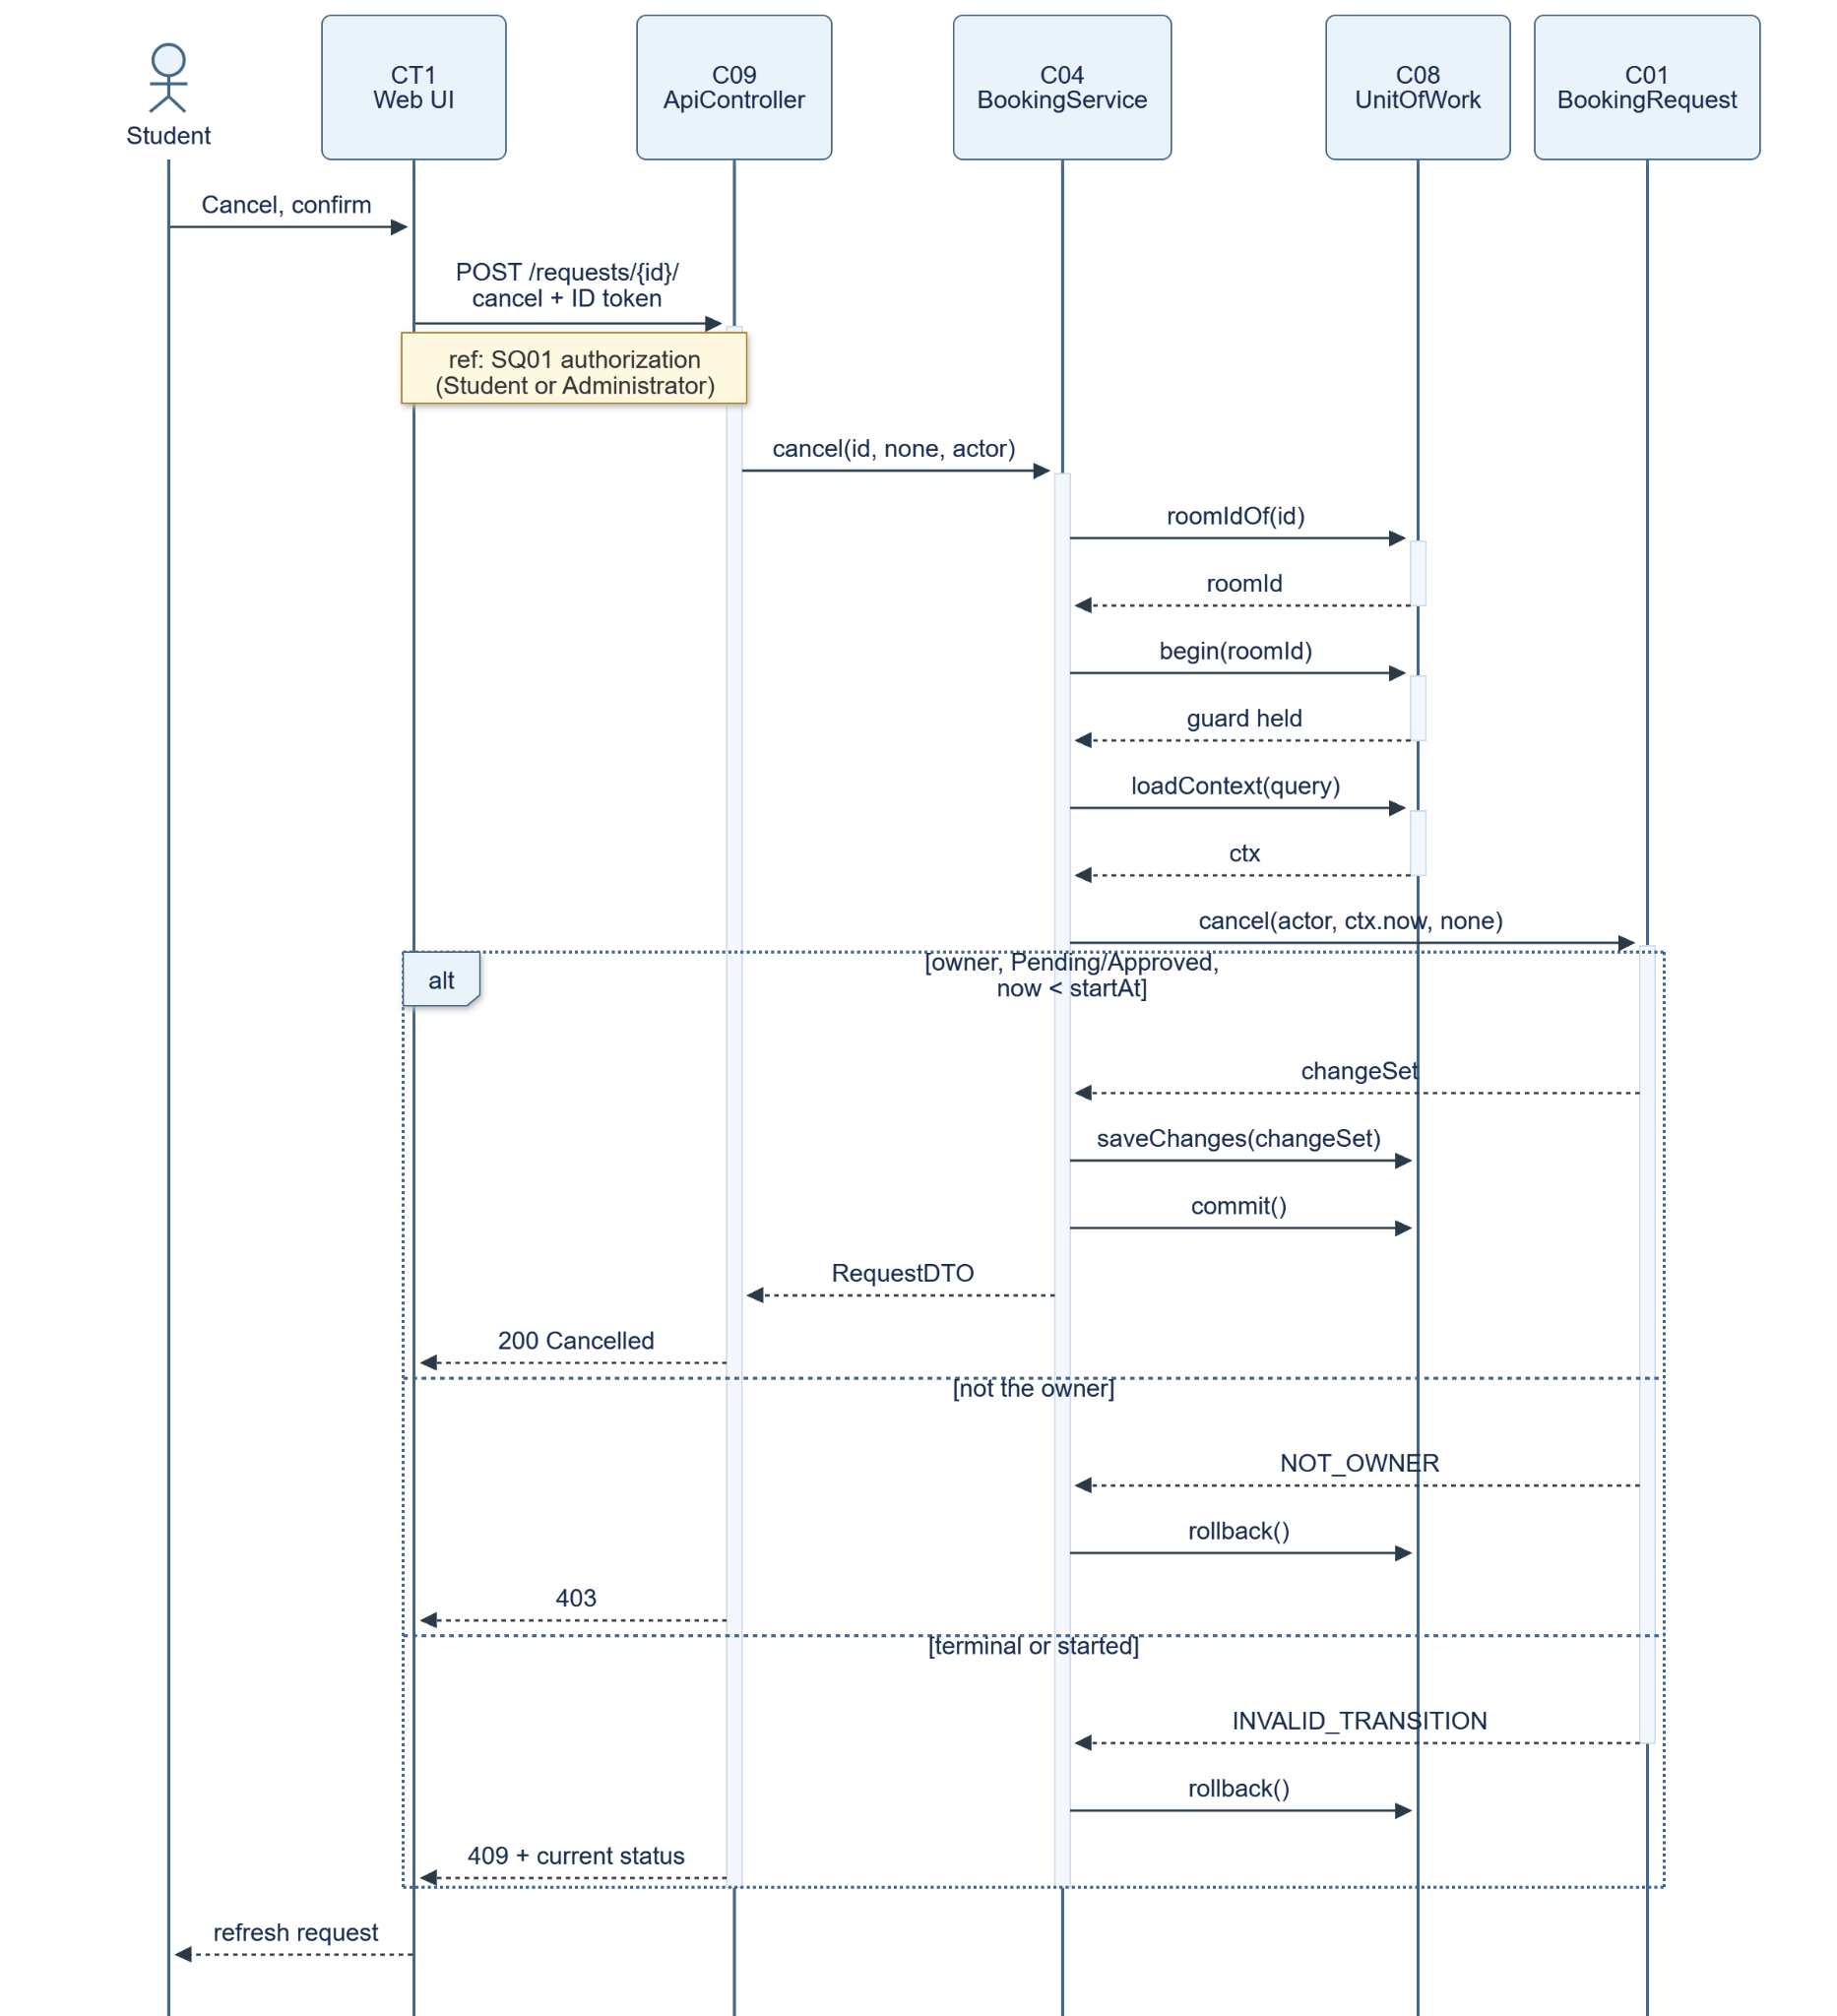
\includegraphics[width=0.94\textwidth,height=0.60\textheight,keepaspectratio]{images/05-object-oriented-design/figure_08.png}
\end{center}
\roomfourfigurecaption{SQ03}{UC-06 owner cancellation; UC-10 reuses the same operation for an Administrator.}
\par\medskip

C01.cancel checks the server-derived actor, the current status and now < startAt using ctx.now. Cancelling an Approved request deletes only its own occupancy row. A request owned by another student returns 403 without record data; a Rejected, Cancelled or started request returns 409 with its current status. UC-10 calls the same operation with an Administrator actor, which is limited to Approved bookings and requires a reason.\par

\subsubsection{SQ04 UC-11 Edit room details}

\par\medskip
\begin{center}
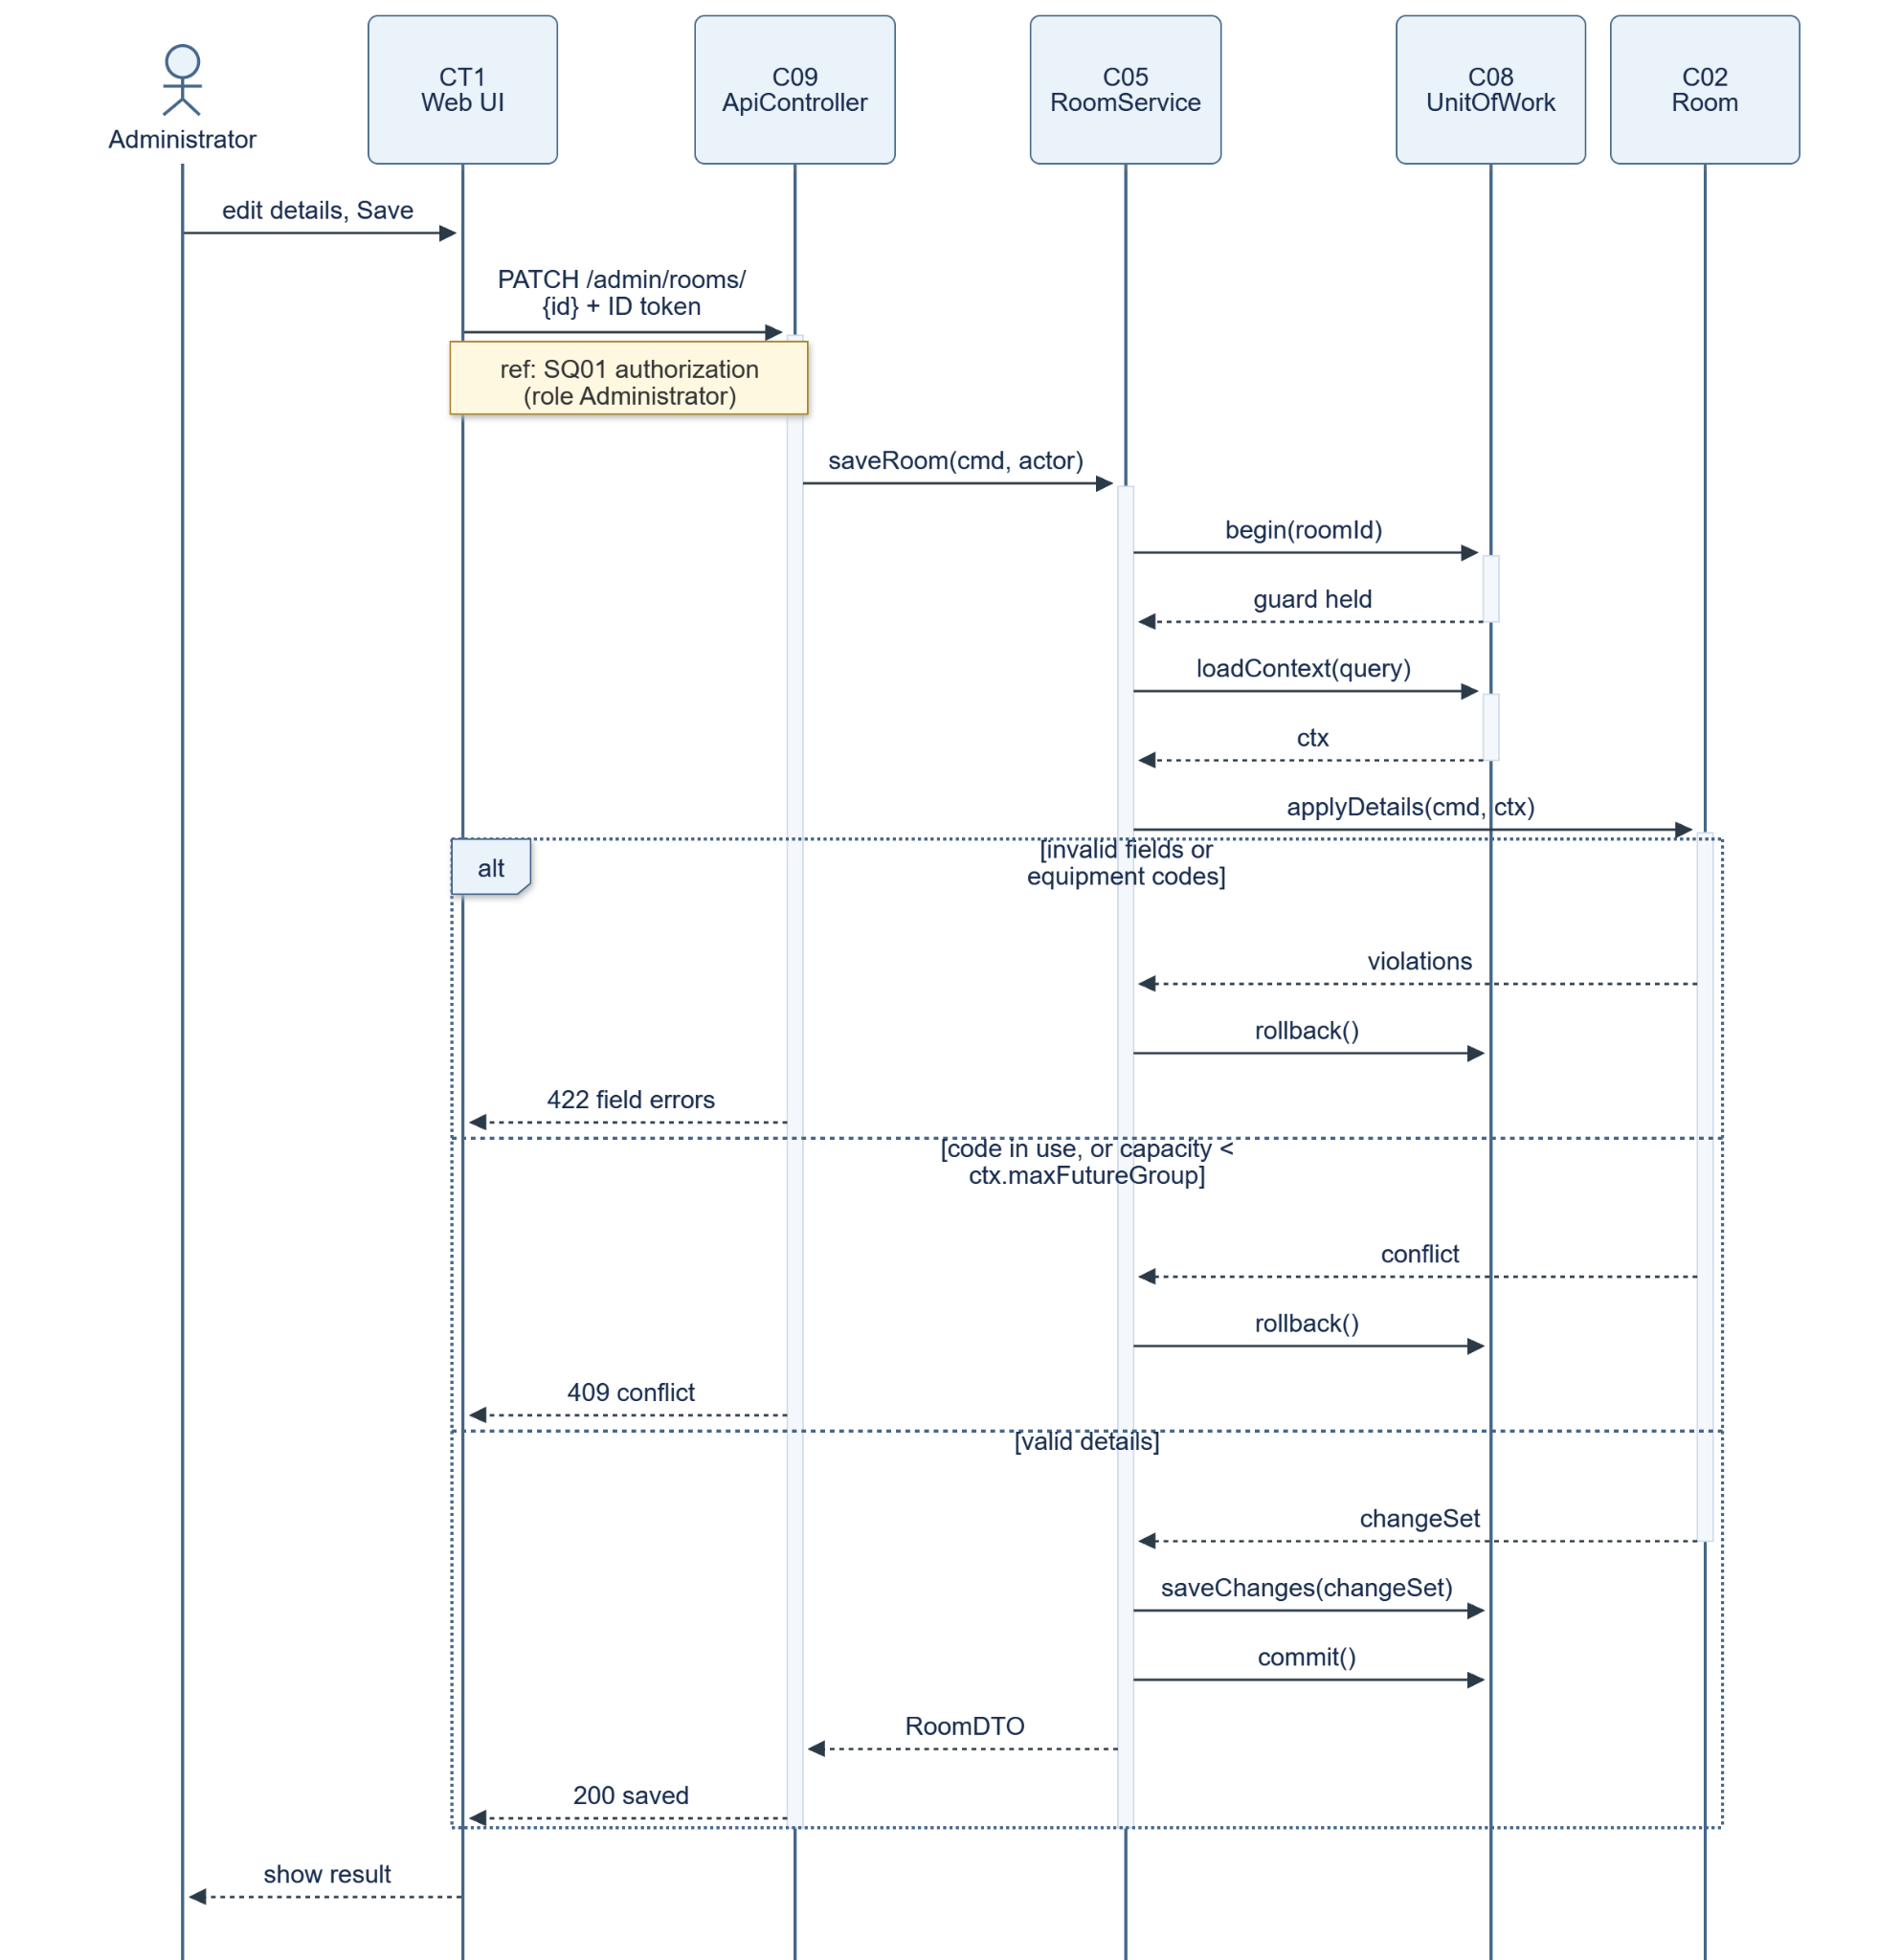
\includegraphics[width=0.94\textwidth,height=0.60\textheight,keepaspectratio]{images/05-object-oriented-design/figure_09.png}
\end{center}
\roomfourfigurecaption{SQ04}{UC-11 save-time room edit, including the capacity check against future Approved bookings.}
\par\medskip

query returns the largest group size among the room's future Approved bookings and whether the normalized code belongs to another room. Because approval waits on the same room guard, either ordering preserves invariant I05: an approval that commits first is included in maxFutureGroup, and an edit that commits first is the capacity the approval checks. A concurrent creation of a different room with the same code is not serialized by this guard; the normalized unique index rejects it at saveChanges (23505 → 409). Creating a new room uses begin(null) and C02.create.\par

\subsubsection{SQ05 UC-13 Create maintenance block}

\par\medskip
\begin{center}
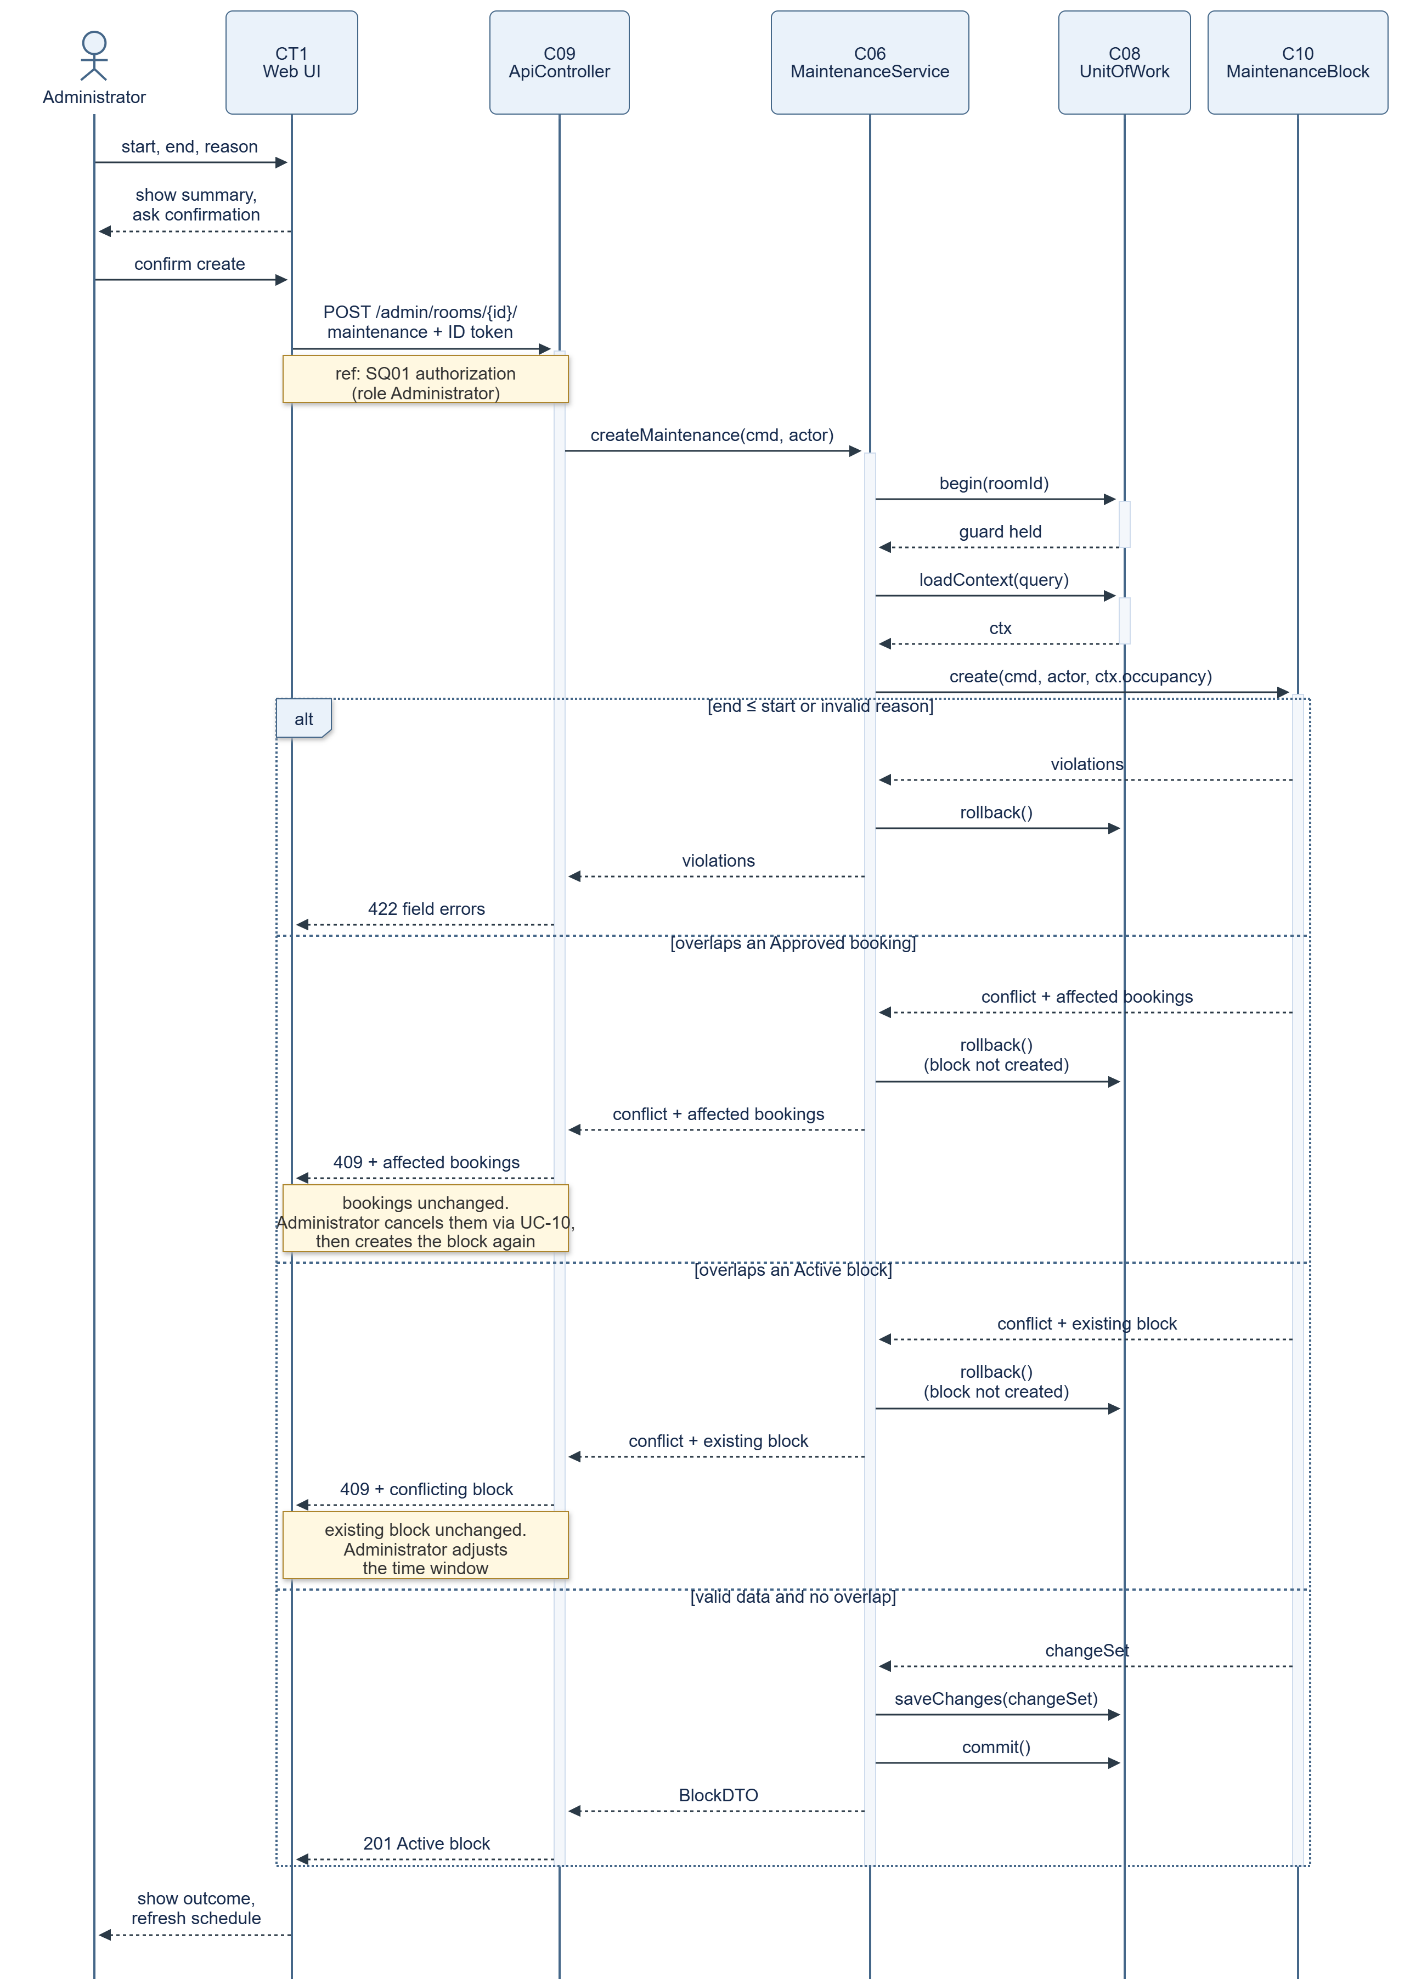
\includegraphics[width=0.94\textwidth,height=0.60\textheight,keepaspectratio]{images/05-object-oriented-design/figure_10.png}
\end{center}
\roomfourfigurecaption{SQ05}{UC-13 maintenance creation without automatic booking cancellation.}
\par\medskip

C10.create validates the window and reason, then checks overlap against Approved bookings and active blocks in ctx.occupancy. Each conflict rolls back and returns HTTP 409 with error.code = SCHEDULE\_CONFLICT, error.requestId and error.conflicts. Following SQ05, if Approved bookings overlap, conflicts lists those bookings first; each item has kind = approved\_booking, bookingRequestId, startAt and endAt. Only when no Approved booking overlaps does conflicts contain the overlapping active maintenance block, with kind = maintenance\_block, maintenanceBlockId, startAt and endAt. S08 can link booking conflicts to UC-10, where the Administrator handles each eligible booking separately before creating the block again; no booking is cancelled automatically (BR-15). A maintenance-block conflict leaves the existing block unchanged so that the Administrator can choose another time window. Removal (UC-13 A1) follows the same frame: roomIdOf(block), begin, loadContext, C10.remove(actor, ctx.now), saveChanges and commit. It marks the block removed with remover and time, deletes only its occupancy row and returns 409 at or after the block start.\par

\subsection{State machine diagrams}

\par\medskip
\begin{center}
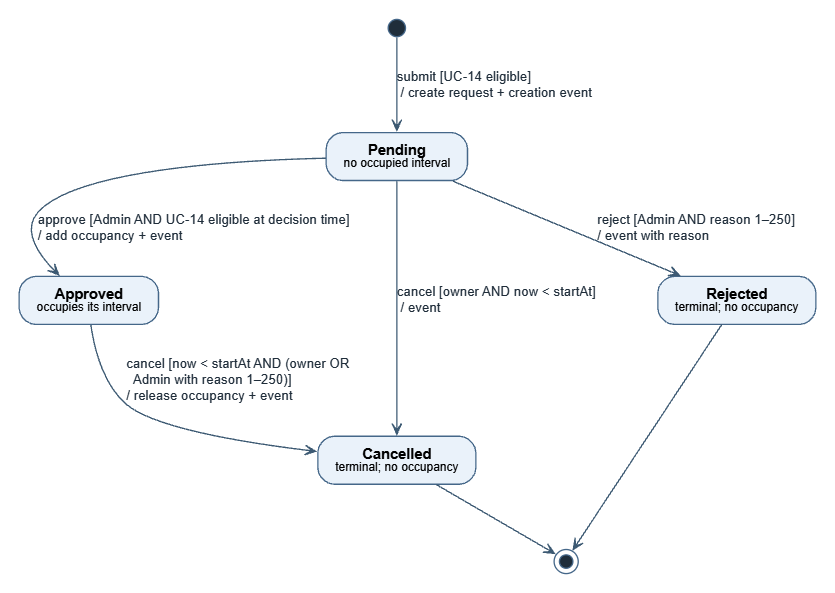
\includegraphics[width=0.94\textwidth,height=0.60\textheight,keepaspectratio]{images/05-object-oriented-design/figure_11.png}
\end{center}
\roomfourfigurecaption{U05}{BookingRequest states. Transitions are written event [guard] / action; Rejected and Cancelled are final.}
\par\medskip

Guards are evaluated at decision time after the room lock, and each successful transition appends exactly one event. The five transitions are the only previous/new status pairs allowed in booking\_events (Section 6). No transition is triggered by time alone: a Pending request whose start has passed stays Pending until an Administrator rejects it, and an Approved booking stays Approved after its interval as history. There is no Expired, Completed, check-in or no-show state. A refused transition leaves the state unchanged and records no event.\par

\par\medskip
\begin{center}
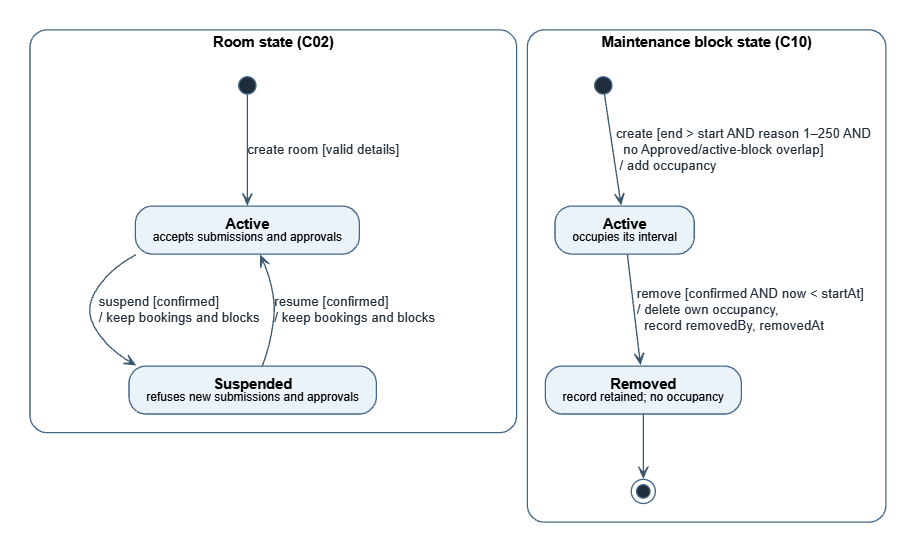
\includegraphics[width=0.94\textwidth,height=0.60\textheight,keepaspectratio]{images/05-object-oriented-design/figure_12.png}
\end{center}
\roomfourfigurecaption{U06}{Independent room and maintenance block states.}
\par\medskip

Suspending or resuming a room never changes bookings, blocks or occupancy (BR-11). A maintenance block that has passed its end time remains active as history; only removal before its start changes its state. Removed is final and the block record is kept.\par

\subsection{Design principles and patterns}

\small
\setlength{\tabcolsep}{3pt}
\renewcommand{\arraystretch}{1.12}
\begin{longtable}{|p{0.23\textwidth}|p{0.31\textwidth}|p{0.38\textwidth}|}
\hline
\textbf{Principle or pattern} & \textbf{Applied at} & \textbf{Reason and limit} \\ \hline
\endfirsthead \hline
Layering, low coupling & C09 → C04–C07, C14 → C01–C03, C10 → C08 & Domain classes import no Express, pg or Firebase code, so rules stay testable. Costs extra interfaces. \\ \hline
Single responsibility, high cohesion & C03 decides eligibility; C04–C06 orchestrate; C08 persists; C14 reads & Each class has one reason to change; avoids a booking "god class". \\ \hline
Information expert, guarded transitions & C01, C02, C10 & Entities own their legal transitions; there is no generic status PATCH. Not the GoF State pattern: four states and one owner make guarded methods simpler (KISS, YAGNI). \\ \hline
Dependency inversion & uowFactory, policy and clock in services; AccountRepository and ReadRepository interfaces & PA4 unit tests can use fakes and a fixed clock for boundaries (08:00, 20:00, now + 7 days) without Firebase or a database. \\ \hline
Unit of Work and Repository & C08 & One client per command: request, occupancy and events commit or roll back together (I01–I06). All writers must use it. \\ \hline
Factory method & Static create on C01, C02, C10; uowFactory & Initial state and creation event are set in one place. \\ \hline
Adapter & C12 & Isolates the Firebase Admin SDK; changing the identity provider affects one class. \\ \hline
Facade & C08 & Hides the pg client, SQL and constraint-error mapping behind seven operations. \\ \hline
Explicit DTO projection & C14 and response DTOs & Privacy follows the returned fields as well as route checks (BR-16, I08). \\ \hline
Idempotent command & C04.submit, C01.matchesSubmission & One logical submission produces one request and one event, even after a lost response (ADR-004). \\ \hline
DRY & TimeInterval.overlaps & One implementation of BR-06 is shared by booking eligibility and maintenance conflicts. \\ \hline
\end{longtable}
\normalsize